\chapter{Automatic Graphic User Interface Generator (AGG)}
	\label{sec:AGG}
	
	La complejidad del sistema implementado en la FPGA en base al código generado por parte del ACG es tal que se vuelve indispensable contar con una herramienta gráfica que facilite la interpretación de los resultados. A su vez, es importante contar con una herramienta que pueda establecer la comunicación con la FPGA, tanto para enviar cómo para recibir las tramas de mensajes definida en la Sección \ref{sec:UART}. Para lograr estos objetivos se creó el AGG (del inglés, Automatic Graphic User Interface Generator), una herramienta diseñada e implementada por el autor de esta tesis de doctorado. El AGG permite establecer la comunicación con la FPGA y actualizar en tiempo real el estado de una interfaz gráfica basada en railML, intuitiva y a semejanza de una consola de señalamiento real.
	
	El AGG utiliza la biblioteca tkinter \cite{TKINTER} para implementar la interfaz gráfica de usuario y la biblioteca serial, nativa de Python, para establecer la comunicación con la plataforma FPGA. La interfaz gráfica se genera utilizando la información provista por el RNA (ver Sección \ref{sec:Biblioteca}), como por ejemplo la topología (posición, conexión y largo de las vías), la distribución de la infraestructura estática (plataformas, final de vías), la disposición de la infraestructura dinámica (cambios de vías, pasos a nivel) y el señalamiento (posición y orientación de las señales). El estado de la interfaz gráfica se actualiza en tiempo real y es reportado a la FPGA en una trama de datos, que ya fue explicada en la Sección \ref{sec:UART}.
	
	El usuario u operario puede interactuar con la interfaz creada mediante tres acciones: hacer zoom in/out utilizando la rueda del mouse, desplazarse por la interfaz arrastrando la topología mientras se mantiene presionada la tecla shift y haciendo click sobre los elementos de la interfaz que son interactivos. los elementos interactivos son aquellos en los cuales hacer click modifica su estado, por ejemplo un cambio de vías, un paso a nivel o una vía. Los finales de vías no poseen estados y, por lo tanto, no son interactivos. Las tres acciones fueron implementadas por el autor de esta tesis de doctorado mediante interrupciones, para tener una respuesta lo más cercana posible a tiempo real. 
	
	Las interacciones producto de hacer click sobre los elementos de la interfaz se dividen en dos tipos de eventos: estáticos y dinámicos. Un evento estático involucra al usuario modificando el estado de la infraestructura, por ejemplo: ocupando o liberando una vía, cerrando o abriendo un paso a nivel o modificando la posición de un cambio de vías. Todas estas acciones se pueden realizar con un click sobre el elemento que se desea modificar. El AGG informará a la FPGA del nuevo estado del elemento seleccionado y actualizará el color y/o posición del elemento, en base a la respuesta de la FPGA. Los colores de cada elemento representan lo siguiente:
		
	\begin{itemize}
		\item Vías: negro (libre), rojo (ocupada), gris (enclavada).
		\item Paso a nivel: azul (abierto), rojo (cerrado), rojo oscuro (enclavado).
		\item Cambio de vías: negro (libre), gris (enclavado).
	\end{itemize}
	
	Debido a que los elementos del sistema de enclavamientos reciben los datos en paralelo, el sistema no converge en un solo ciclo. Supongamos un caso muy común en un señalamiento: dos señales A y B, tal que A depende del estado de B, por pertenecer al recubrimiento (ver Sección \ref{sec:function_5}), y ambas dependen de la trama de entrada. Al recibir la misma trama a la vez, ambas señales evolucionarán de un estado inicial a un estado final, pero la señal A lo hará utilizando la información del estado inicial de B, que ya no sería válido si B cambió de estado. Para evitar esto, el AGG compara la trama de datos enviada a la FPGA con la trama de datos recibida desde la FPGA. Si las tramas son idénticas entonces el sistema de enclavamientos ya ha alcanzado un estado de equilibrio y el AGG detendrá el envío de datos hasta que el operador altere ese equilibrio interactuando con la interfaz. En cambio, si las tramas de datos son diferentes, el AGG enviará a la FPGA la trama recibida, junto con los pedidos que el usuario pudiese haber solicitado entre ambos sucesos. De esta forma, el AGG cierra el lazo de control con la FPGA reinyectando las tramas de datos hasta que las tramas de datos converjan y se cumpla la convergencia.

	\section{Representación de cada elemento ferroviario en la interfaz gráfica}
	\label{sec:AGG_STATUS}
	
	Ejemplo de cada cosa
	
	Vías
	
	\begin{figure}[H]
		\centering
		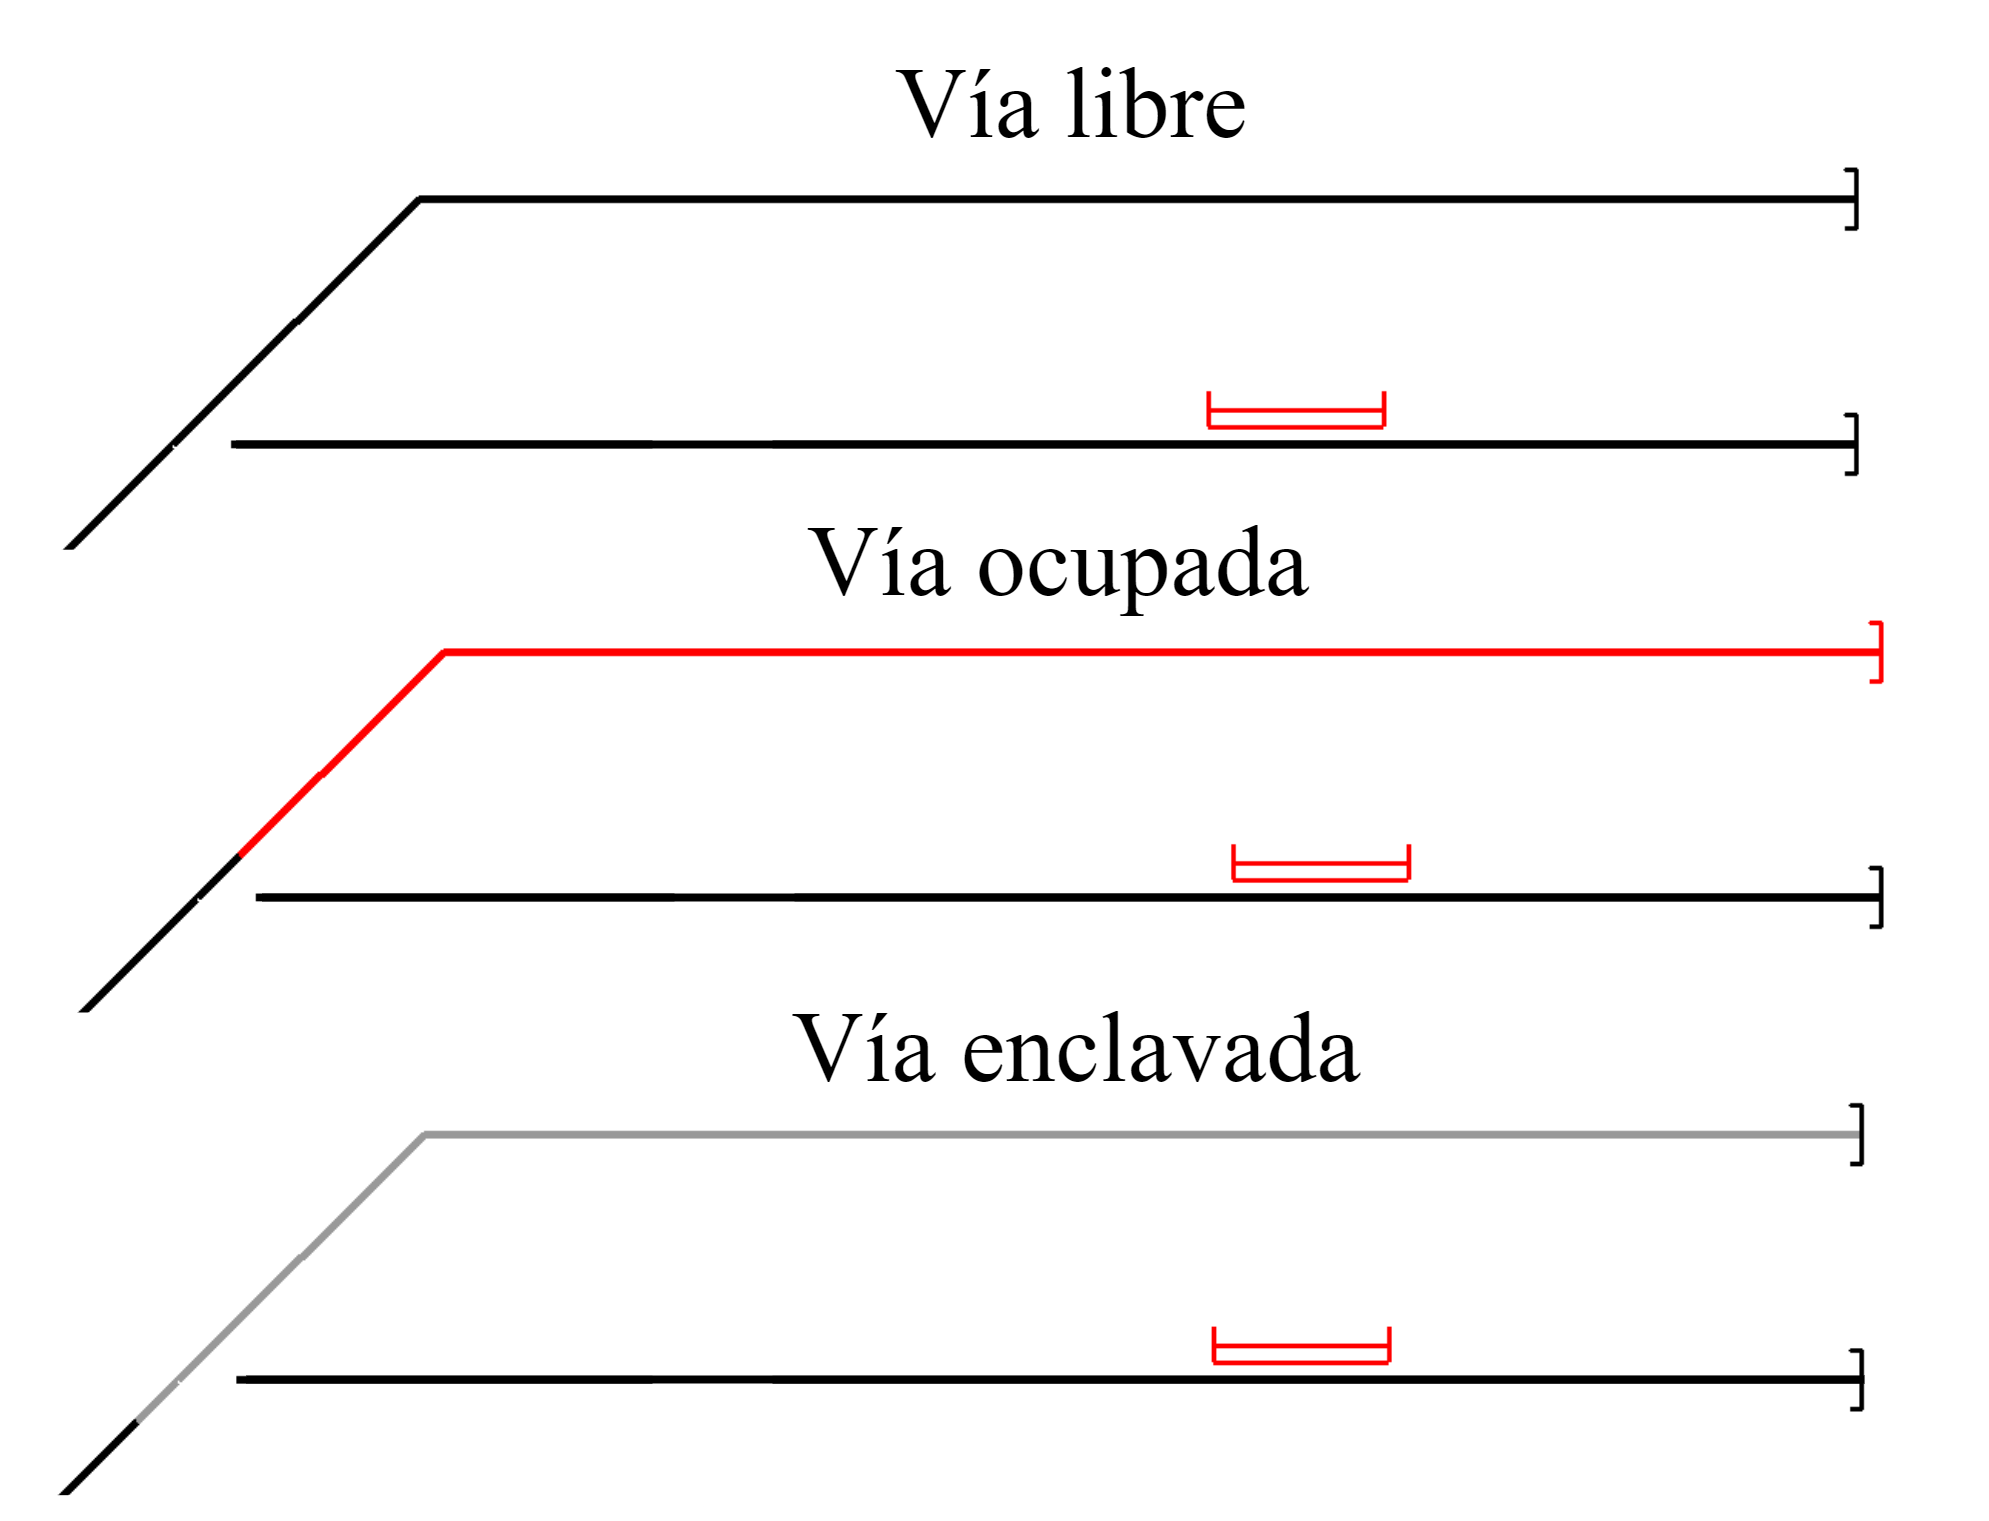
\includegraphics[width=0.7\textwidth]{AGG/images/AGG_via}
		\centering\caption{Interfaz gráfica del ejemplo 1.}
		\label{fig:AGG_tracks}
	\end{figure}
	
	Paso a nivel
	
	\begin{figure}[H]
		\centering
		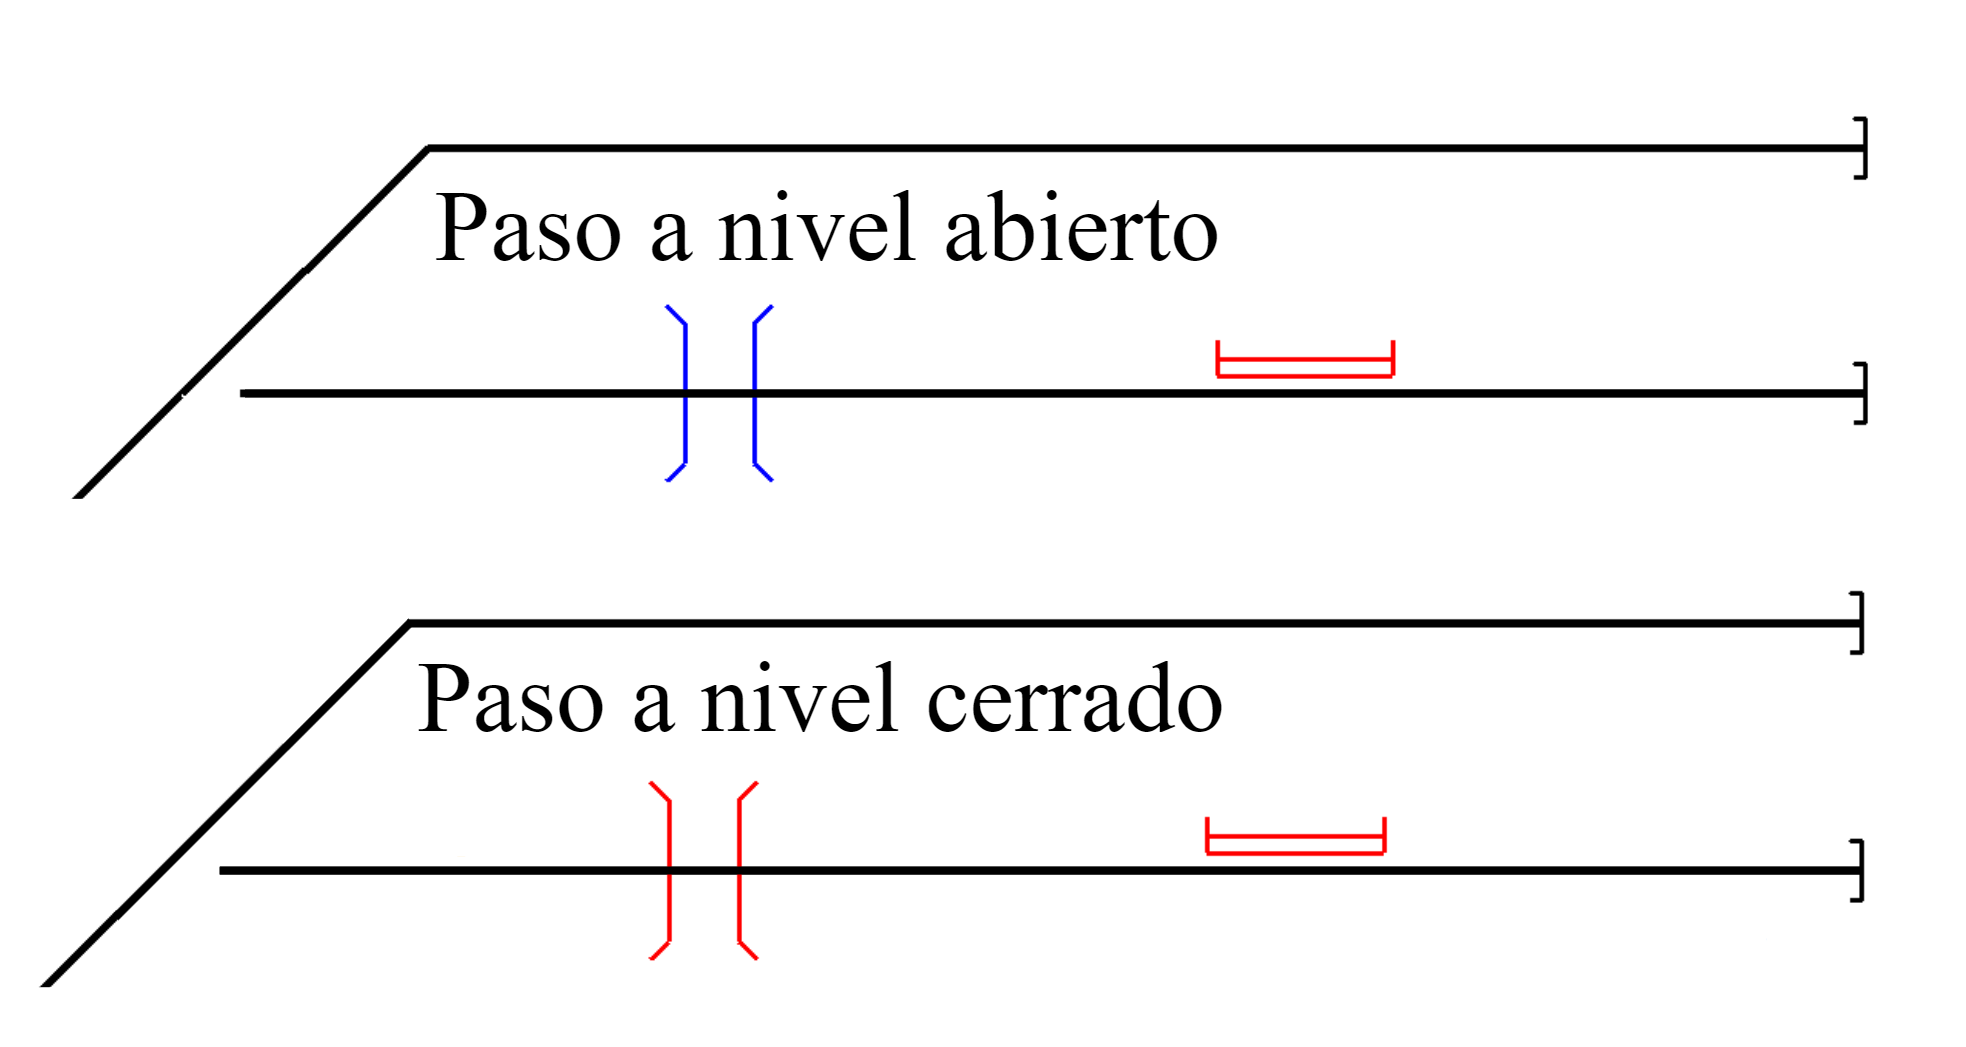
\includegraphics[width=0.7\textwidth]{AGG/images/AGG_cruce}
		\centering\caption{Interfaz gráfica del ejemplo 1.}
		\label{fig:AGG_levelCrossing}
	\end{figure}
	
	
	
	Cambio de vias simple
	
	\begin{figure}[H]
		\centering
		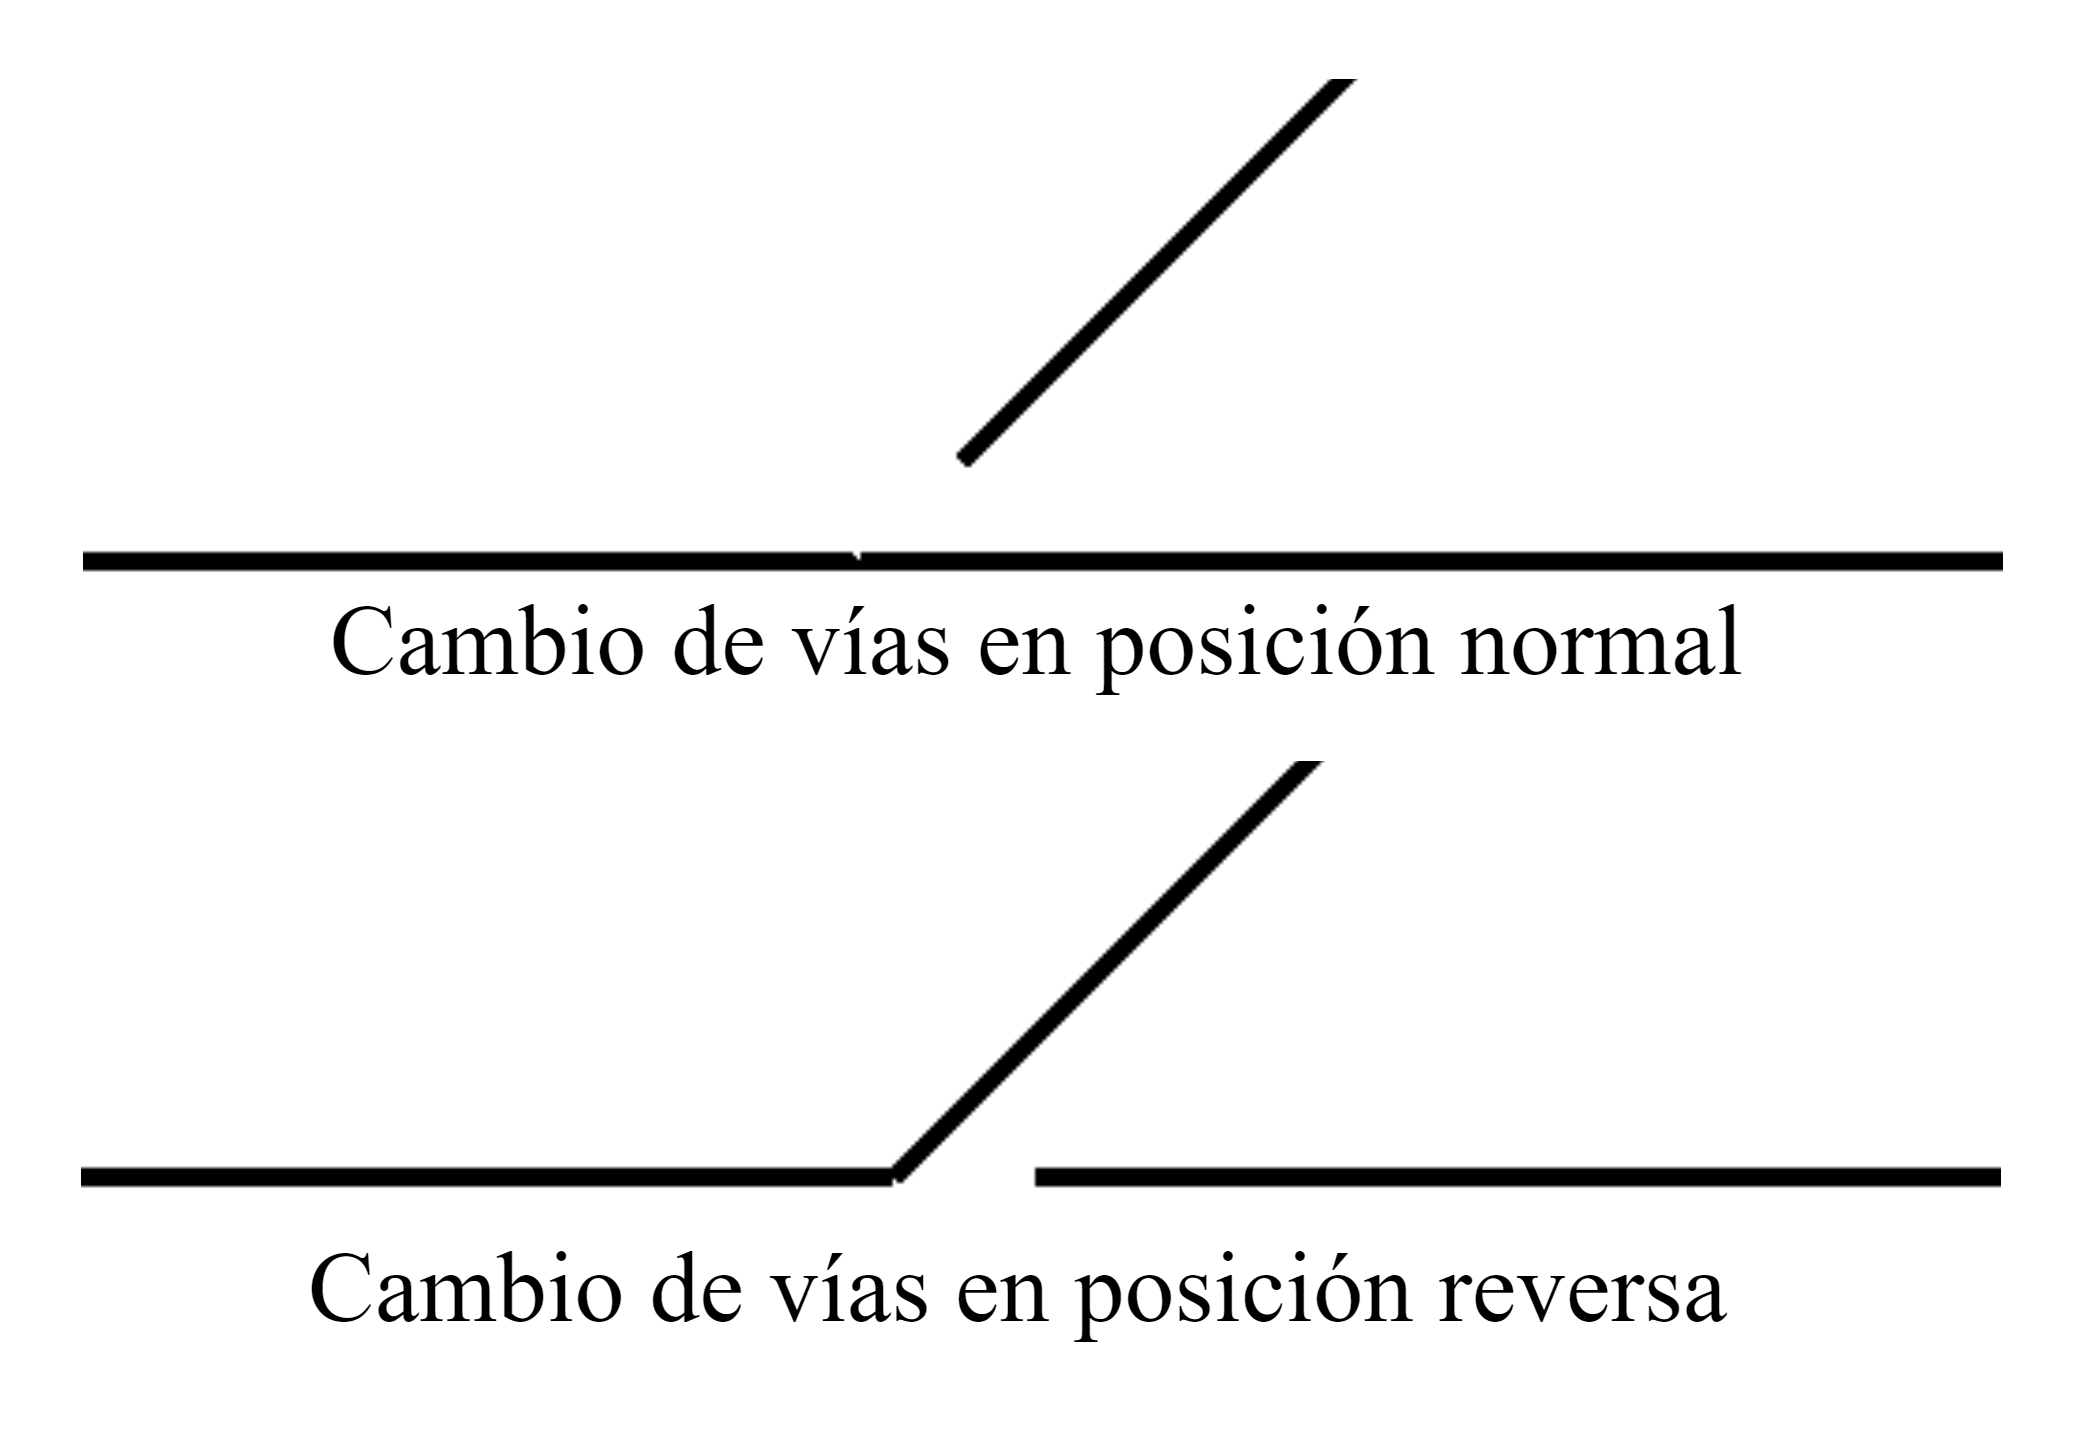
\includegraphics[width=0.7\textwidth]{AGG/images/AGG_switch}
		\centering\caption{Interfaz gráfica del ejemplo 1.}
		\label{fig:AGG_switch}
	\end{figure}

	
	Ruta seleccionada
	
	Ruta solicitada
	
	\begin{figure}[H]
		\centering
		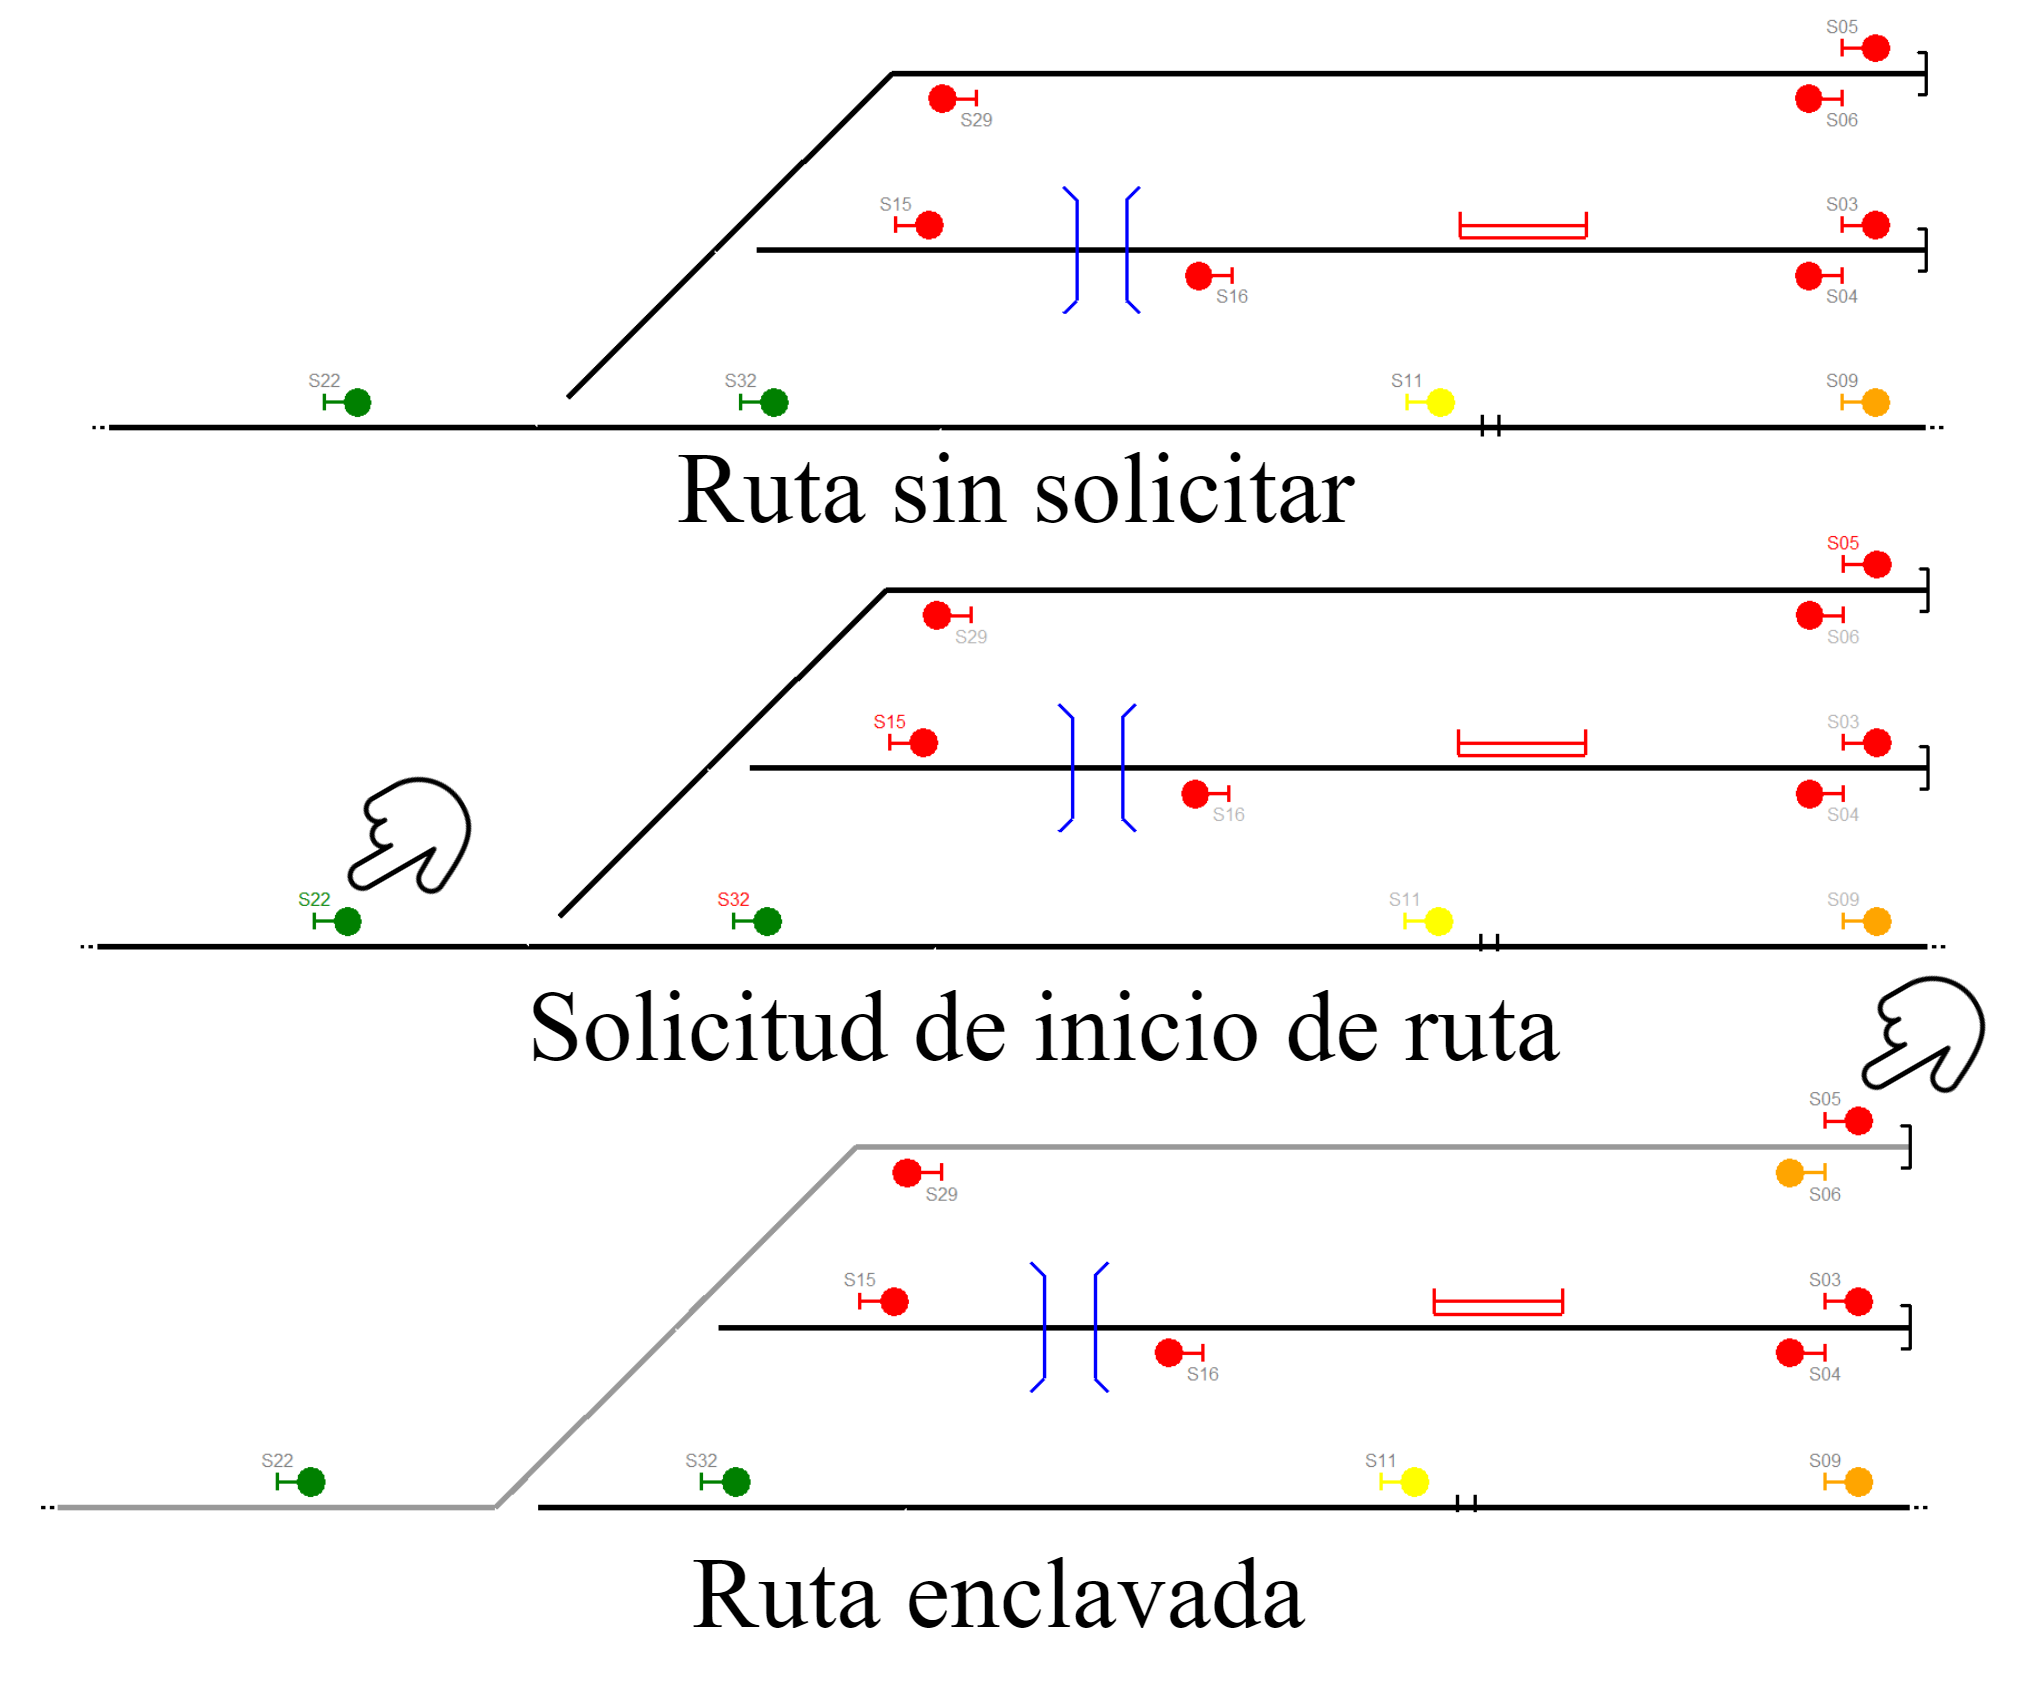
\includegraphics[width=0.7\textwidth]{AGG/images/AGG_routes}
		\centering\caption{Interfaz gráfica del ejemplo 1.}
		\label{fig:AGG_routes}
	\end{figure}
	
		
	
	



	